\subsection*{Appendix A.3}
If income changes, the budget constraint will shift.\\
Depending on the new optimum, good 1 or 2 may be normal goods or inferior goods.\\
If you connect all the optimal points, you get the \emph{income offer curve}.
\begin{figure}[H]
    \centering
    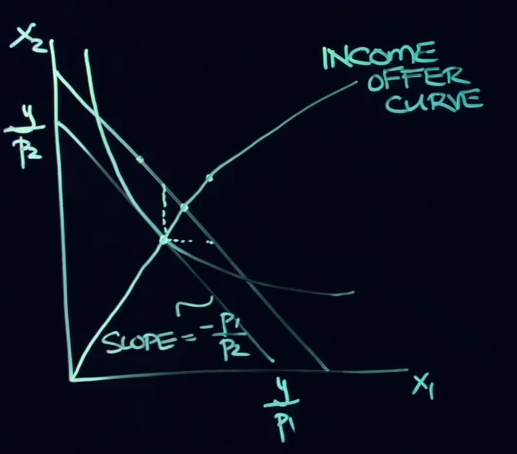
\includegraphics[width=0.5\textwidth]{Chapter6/IncomeChanges.png}
    \caption{Income Offer Curve}
    \label{fig:Income_Offer_Curve}
\end{figure}
If the price of good 1 changes, the budget constraint's slope will change.
If we connect all the optimal points, we get the \emph{price offer curve}.
\begin{figure}[H]
    \centering
    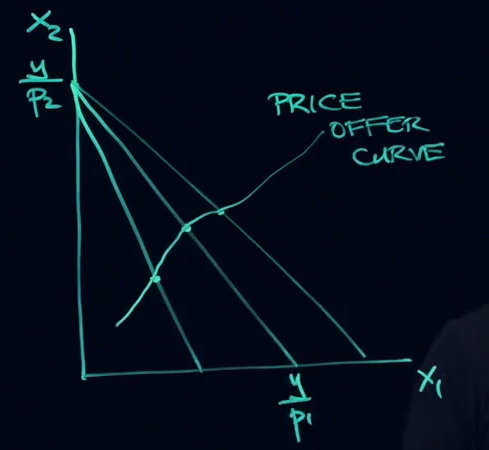
\includegraphics[width=0.5\textwidth]{Chapter6/PriceChanges.png}
    \caption{Price Offer Curve}
    \label{fig:Price_Offer_Curve}
\end{figure}